\documentclass[aspectratio=169]{beamer}
\usepackage{tikz}
\usepackage{graphicx}
\usepackage{listings}

\usecolortheme{whale}
\usetikzlibrary{er,positioning}  
\usetikzlibrary{decorations.pathreplacing}
\usetikzlibrary{arrows, decorations.markings}
\usetikzlibrary{shapes.geometric}
\usetikzlibrary{shapes.arrows}
\usetikzlibrary{overlay-beamer-styles}

% \setbeameroption{show notes on second screen=left}

\setbeamertemplate{navigation symbols}{}

\tikzstyle{every link} = []
\tikzstyle{link} = [>=triangle 60, draw, every link]

\definecolor{attr}{RGB}{10,153,2}

\title{Bases de Datos}
\subtitle{Modelaci\'on Conceptual}
\author[Garc\'ia L., Cardentey V. M., Ledesma A.]{
    Lic. Andy Ledesma Garc\'ia\\
    Lic. V\'ictor M. Cardentey Fundora\\ 
    Dra. C. Lucina Garc\'ia Hern\'andez
}
\institute[MATCOM-UH]{
    Departamento de Computaci\'on\\
    Facultad de Matem\'atica y Computaci\'on\\
    Universidad de La Habana\\[3mm]
    Licenciatura en Ciencia de Datos
}
\date[]{30 de enero de 2024}


\begin{document}
    \maketitle
    
\definecolor{blue1}{RGB}{126,126,206}
\definecolor{blue2}{RGB}{87,87,192}
\definecolor{blue3}{RGB}{51,51,178}
\definecolor{blue4}{RGB}{27,26,107}

\begin{frame}{Procesamiento de datos}
    \begin{overlayarea}{\linewidth}{\textheight}
        \vspace{5mm}
        \centering
        \begin{tikzpicture}
            \node[rectangle, fill=blue1, minimum width=5cm, minimum height=8mm, text=white] at (0,0) {An\'alisis de Requerimientos};
            \node[single arrow, fill=black, inner sep=6pt, rotate=270] at (0,-0.8){};
            \node[rectangle, fill=blue2, minimum width=5cm, minimum height=8mm, text=white] at (0,-1.8) {Modelos Conceptuales};
            \node[single arrow, fill=black, inner sep=6pt, rotate=270] at (0,-2.6){};
            \node[rectangle, fill=blue3, minimum width=5cm, minimum height=8mm, text=white] at (0,-3.6) {Bases de Datos};
            \node[single arrow, fill=black, inner sep=6pt, rotate=270] at (0,-4.4){};
            \node[rectangle, fill=blue4, minimum width=5cm, minimum height=8mm, text=white] at (0,-5.4) {Consultas};
        \end{tikzpicture}
    \end{overlayarea}
        
    \note{@NOTE se levantan los requerimientos y se analizan. En esta semana vamos a ver los 2 1ros}
\end{frame}

    \begin{frame}
    \frametitle{Metodolog\'ia}

    \begin{columns}
        \column{.45\textwidth}

        \includegraphics<1-2>[width=\textwidth]{img/specs-and-dbs.jpg}
        \includegraphics<4-6>[width=\textwidth]{img/the-thinker.jpg}
        \includegraphics<8>[width=\textwidth]{img/presenting-data.png}

        \column{.1\textwidth}
        \begin{center}
            
\begin{tikzpicture}
                \node<2,6>[single arrow, fill=black, inner sep=6pt] at (0,0){};
                \node<4,8>[single arrow, fill=black, inner sep=6pt, rotate=180] at (0,-1){};
            \end{tikzpicture}
        \end{center}

        \column{.45\textwidth}
            \only<2-4>{
            \resizebox{\textwidth}{!}{
                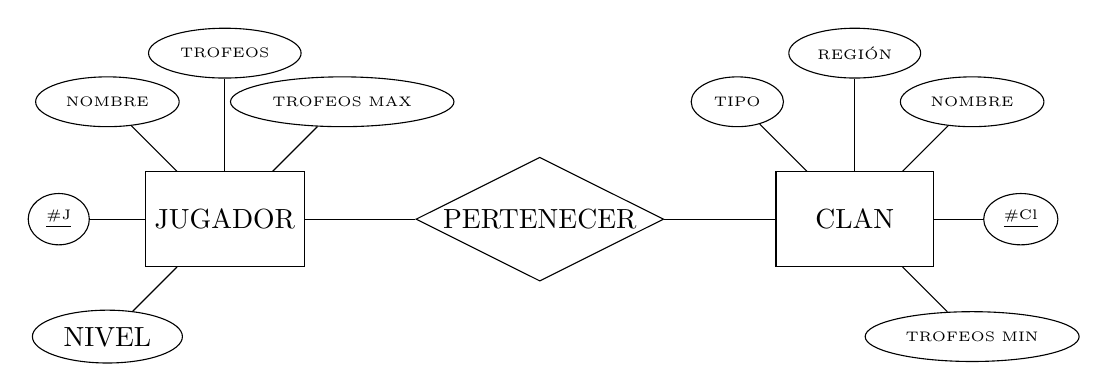
\begin{tikzpicture}[node distance=6em]
                    \tikzstyle{every entity} = [minimum width=2cm, minimum height=1.2cm]
                    \node[entity] (jugador) {JUGADOR}
                        [sibling distance=3cm]
                        child {node[attribute] [above right of=jugador] {\tiny TROFEOS MAX}}
                        child {node[attribute] [above of=jugador] {\tiny TROFEOS}}
                        child {node[attribute] [above left of=jugador] {\tiny NOMBRE}}
                        child {node[attribute] [left of=jugador] {\underline{\tiny \#J}}}
                        child {node[attribute] [below left of=jugador] {NIVEL}}
                        ;
                  
                    \node[entity] (clan) at (8,0) {CLAN}
                    [sibling distance=3cm]
                    child {node[attribute] [right of=clan] {\underline{\tiny \#Cl}}}
                    child {node[attribute] [above of=clan] {\tiny REGI\'ON}}
                    child {node[attribute] [above left of=clan] {\tiny TIPO}}
                    child {node[attribute] [above right of=clan] {\tiny NOMBRE}}
                    child {node[attribute] [below right of=clan] {\tiny TROFEOS MIN}};

                    \node[relationship,aspect=2] (pertenecer) at (4,0) {PERTENECER}
                    edge(jugador) edge(clan);
                \end{tikzpicture}
            }

            }
            \includegraphics<6-8>[width=\textwidth]{img/dev-interacts-bds.png}
    \end{columns}
\end{frame}
    \begin{frame}{En resumen... nuestro prop\'osito}
    \begin{columns}
        \column{0.45\linewidth}
            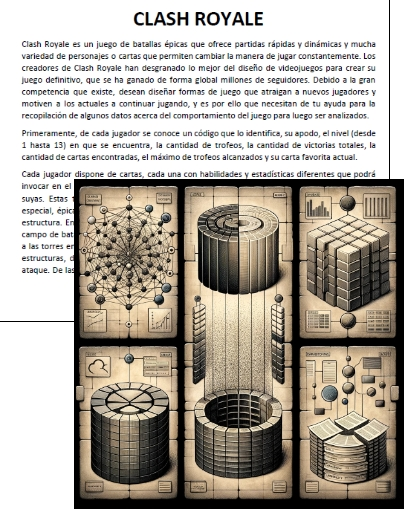
\includegraphics[width=\linewidth]{img/specs-and-dbs.jpg}
            
        \column{.1\linewidth}
            \begin{center}
                
\begin{tikzpicture}
                    \node[single arrow, fill=black, inner sep=6pt] at (0,0){};
                \end{tikzpicture}
            \end{center}
            
        \column{0.45\linewidth}
            
\includegraphics[width=\linewidth]{img/presenting-data.png}
        
    \end{columns}

    \note{@NOTE fin de parte. Pregunta dudas}
\end{frame}

\begin{frame}{Descripci\'on de la realidad}
    \begin{block}{¿C\'omo es una descripci\'on de la realidad?}
        \begin{enumerate}
            \item<2-> Est\'a planteada en lenguaje natural (Espa\~nol, Ingl\'es,...)
            \item<3-> Es realizada por personas con distinta formaci\'on y conocimiento
            \item<4-> Contiene una serie de \textcolor{red}{requerimientos informacionales} \begin{itemize}
                \item<5-> ¿Qu\'e datos ser\'ia de inter\'es almacenar?
                \item<6-> ¿Qu\'e restricciones o reglas se establecen sobre estos datos?
                \item<7-> ¿Qu\'e preguntas se quieren responder utilizando los datos almacenados?
            \end{itemize}
            \item<8-> Puede estar basada en cualquier \'area de la actividad humana
        \end{enumerate}
        
    \end{block}
\end{frame}
    
{
    \setbeamertemplate{background}{
        
\includegraphics[width=\paperwidth, height=\paperheight]{img/coc.jpg}
    }
    \begin{frame}
    \end{frame}
}


\begin{frame}{¿Qu\'e es Clash Royale?}

    \onslide<1->{
        \begin{block}{}
            Clash Royale es un juego social de estrategia en tiempo real donde los jugadores
            pueden hacer amigos, pertenecer a un clan y coleccionar cartas para enfrentarse
            con otros jugadores en \'epicas batallas de defensa de torres.
        \end{block}
    }

    \onslide<2>{
        \vspace{5mm}

        \begin{center}
        \Large \textcolor{red}{¿C\'omo modelar este escenario a partir de la especificaci\'on?}
            
        \end{center}
    }

    \note<2>{@NOTE esta especificaci\'on es para los datos y sus v\'inculos}
\end{frame}

    

\begin{frame}{Motivaci\'on}
    \begin{columns}[T]
        \begin{column}{0.48\linewidth}
            \centering
            \begin{tikzpicture}
                \node[inner sep=0pt] at (1.4,5.8) {
                    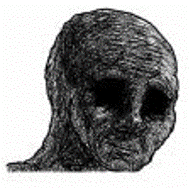
\includegraphics[width=2cm]{img/sface.png}
                };
        
        
                \node[inner sep=0pt] at (1.4,3.2) {
                    
\includegraphics[width=2cm]{img/hface.png}
                };
        
                \draw[-,thick] (0.3, 4.6) -- (6,4.5);
                \draw[-,thick] (2.7, 2) -- (2.7,6.8);
        
                \node[inner sep=0pt] at (4.4, 3.2) {
                    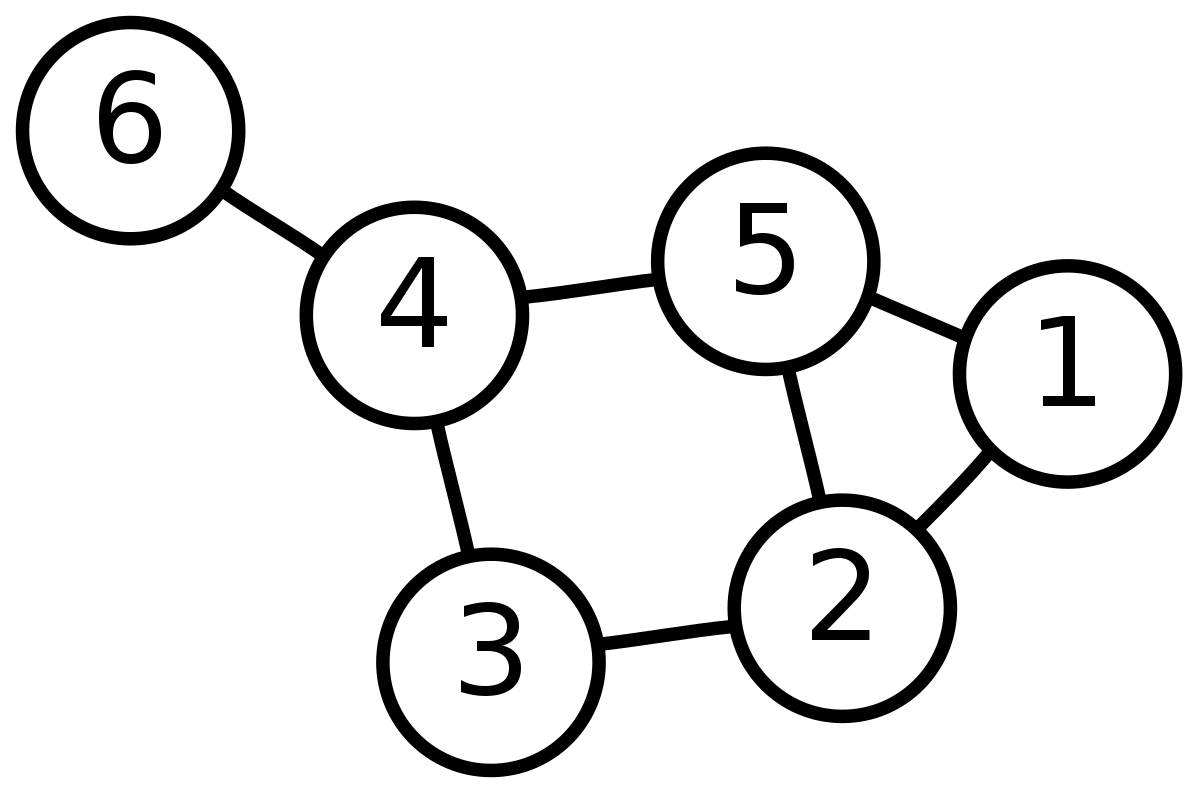
\includegraphics[width=3cm, height=2.5cm]{img/graph.png}
                };

                \node[align=left] at (5, 5.8) {\tiny $G=(V,A)$\\ \tiny $V:$ Conjunto finito de v\'ertices\\ \tiny $A:$ Conjunto de aristas $\{v,w\} : v,w \in V$} ;
        
            \end{tikzpicture}
        \end{column}

        \begin{column}{0.48\linewidth}
            \vspace{15mm}
            Las representaciones visuales permiten que los \textcolor{red}{conceptos} matem\'aticos y
            computacionales abstractos se vuelvan m\'as concretos
        \end{column}
        
    \end{columns}
   
\end{frame}

\begin{frame}{Concepto de base de datos}
    \begin{block}{}
        \begin{quote}
            ``... una base de datos es una colecci\'on auto-descriptiva de registros integrados."
            \hspace{1em plus 1fill}---Allen Taylor
        \end{quote}
    \end{block}

    \note{@NOTE \'enfasis en q lo que se registran son los datos y sus interrelaciones}
\end{frame}

\begin{frame}{¿Y si nos enfocamos en la idea?}

    \onslide<1->{
        \begin{block}{}
            \begin{itemize}
                \item Una base de datos es una colecci\'on de {\color<2>{red}conjuntos de registros} con la {\color<2>{red}misma estructura} entre los que se establecen {\color<2>{red}interrelaciones}.
            \end{itemize}
        \end{block}
    }

    \onslide<2->{
        \begin{alertblock}{Elementos principales}
            \begin{itemize}
                \item Conjuntos de registros
                \item Interrelaciones entre los conjuntos de registros
                \item Estructura de los registros
            \end{itemize}
        \end{alertblock}
    }
\end{frame}
    \begin{frame}{Busquemos estos elementos}
    \begin{overlayarea}{\linewidth}{\textheight}
        \vspace{20mm}
        \begin{block}{}
            Clash Royale es un juego social de estrategia en tiempo real
            donde los {\color<3->{orange} jugadores} pueden {\color<5->{blue} hacer amigos},
            {\color<5->{blue}pertenecer} a un {\color<3->{orange}clan} 
            y {\color<5->{blue} coleccionar} {\color<3->{orange} cartas} para
            {\color<5->{blue} enfrentarse} con otros jugadores en
            \'epicas batallas de defensa de torres.
        \end{block}

        \vspace{5mm}

        \centering
        \only<2>{\Large \textcolor{red}{¿Qu\'e conjuntos de registros ser\'ia importante almacenar?}}
        \only<4>{\Large \textcolor{red}{¿Qu\'e interrelaciones existen entre estos conjuntos?}}
        \note[item]{Welcome to the talk}
    \end{overlayarea}
    
\end{frame}


\begin{frame}{Removiendo lo innecesario}
    \begin{center}
        \Large Hechos que conocemos:
        \vspace{5mm}
        
        \textcolor{orange}{jugador} \hspace{10mm} \textcolor{blue}{ser amigo} \hspace{10mm} \textcolor{orange}{jugador}
        \vspace{5mm}

        \textcolor{orange}{jugador} \hspace{10mm} \textcolor{blue}{pertenecer} \hspace{10mm} \textcolor{orange}{clan}
        \vspace{5mm}

        \textcolor{orange}{jugador} \hspace{10mm} \textcolor{blue}{coleccionar} \hspace{10mm} \textcolor{orange}{carta}
        \vspace{5mm}

        \textcolor{orange}{jugador} \hspace{10mm} \textcolor{blue}{enfrentar} \hspace{10mm} \textcolor{orange}{jugador}
    \end{center}
\end{frame}

    \begin{frame}{¿C\'omo representar estos elementos?}
    \begin{block}{Modelo Entidad-Relacionalidad Extendido (MERX)}
        \begin{itemize}
            \item<1-> Representa conceptualmente las interrelaciones entre conjuntos de inter\'es en un dominio espec\'ifico del conocimiento
            \item<2-> Basado en Teor\'ia de Conjuntos y Programaci\'on Orientada a Objetos
            \item<3-> Es intuitivo
        \end{itemize}
        
        
        % \begin{itemize}
        %     \item Teor\'ia de conjuntos $\to$ L\'ogica
        %     \item Programaci\'on orientada a objetos $\to$ Programaci\'on
        %     \item Intuitiva $\to$ Salvaci\'on
        % \end{itemize}
    \end{block}
\end{frame}
      



\begin{frame}{Modelando conjuntos}
    \begin{block}{}
        \textcolor{orange}{Conjunto de entidades}: Conjunto de objetos que se puedan identificar
        en el escenario que se desea representar y que tienen cierto
        significado para el usuario.

        \vspace{3mm}
        Conjunto: JUGADOR = \{Juan, Marcos, Mar\'ia,...\}
        \vspace{3mm}

        Representaci\'on gr\'afica:

        \vspace{3mm}
        \centering
        
\begin{tikzpicture}
            \node[entity,minimum width=2.3cm, minimum height=1.2cm] (jugador) at (3.2,0) {JUGADOR};
        \end{tikzpicture}
    \end{block}

    \note{@NOTE esta representaci\'on gr\'afica se trata as\'i por convenio}
\end{frame}

\begin{frame}{Modelando interrelaciones}
    \begin{block}{}
        \textcolor{blue}{Conjuntos de interrelaciones}: Un conjunto
        de concatenaciones de instancias tomadas de los conjuntos
        de entidades que se relacionan.

        \vspace{3mm}

        Conjunto: PERTENECER = \{(Juan, TheWarriors), (Pedro, bravehearts), ...\}

        \vspace{3mm}

        Representaci\'on gr\'afica:

        \vspace{3mm}

        \centering
        
\begin{tikzpicture}
            \node[entity,minimum width=2.3cm, minimum height=1.2cm] (jugador) at (3.4,0) {JUGADOR};
            \node[entity,minimum width=2.3cm, minimum height=1.2cm] (clan) at (13,0) {CLAN};
            \node[relationship, aspect=2] at (8.2,0) {PERTENECER} edge(jugador) edge(clan);
        \end{tikzpicture}
        
        \vspace {3mm}

        \onslide<2>{
        \Large \textcolor{red}{¿Qu\'e instancias pertenecen a este conjunto?}
        }

    \end{block}

    \note<1>{@NOTE rombo para $n \leq 4$. Pent\'agono pa $n = 5$, etc}
\end{frame}





    
\begin{frame}{Restricciones sobre interrelaciones}

    \begin{block}{Cardinalidad de una interrelaci\'on}
        Cantidad de instancias en un conjunto de entidades que
        puede estar relacionado con una \'unica instancia en el otro
        conjunto de entidades.
    \end{block}

    \pause

    \begin{block}{¿C\'omo determinar la cardinalidad de una interrelaci\'on?}
        Por cada conjunto de entidades en un extremo de la interrelaci\'on: \begin{enumerate}
            \item Fijar una \'unica entidad en el conjunto de entidades restante
            \item Calcular la cantidad de instancias relacionadas con las entidades fijadas
        \end{enumerate}
    \end{block}
\end{frame}

% One to many relationship example
\begin{frame}
    {
    \only<-9>{Determinar la cardinalidad de una interrelaci\'on. Ejemplo}
    \only<10>{Interrelaciones de uno a muchos}
    }

    \begin{overlayarea}{\linewidth}{\textheight}
        \vspace{10mm}
        \begin{center}
            \Large{
                \textcolor{orange}{jugador} \hspace{10mm} \textcolor{blue}{pertenecer} \hspace{10mm} \textcolor{orange}{clan}
            } 
        \end{center}
        \vspace{3mm}

        \centering
        \begin{tikzpicture}
            \tikzstyle{every entity} = [minimum width=2.3cm, minimum height=1.2cm]
            \node[entity] (jugador) at (0,0) {JUGADOR};
            \node[entity] (clan) at (9,0) {CLAN};
            \node[relationship, aspect=2] (pertenecer) at (4.5,0) {PERTENECER} edge(jugador) edge(clan);
            \onslide<4-8>{\node at (7.5,0.2) {{\color<4,8>{red}{1}}};}
            \only<4>{\draw[->,thick,color=red](7,0.7) -- (7.4,0.4);}
            \onslide<7-8>{\node at (1.5,0.2) {{\color<7,8>{red}{$\ast$}}};}
            \only<7>{\draw[->,thick,color=red](1.9,0.8) -- (1.6,0.4);}
            \onslide<9-10>{\node at (7.5,0.2) {${\color<9>{red}{0}}, 1$};}
            \onslide<9-10>{\node at (1.5,0.2) {${\color<9>{red}{1}}, \ast$};}

        \end{tikzpicture}

        \only<2-4>{
            \begin{block}{Cardinalidad en el extremo CLAN}
                \begin{enumerate}
                    \item Fijamos una \'unica entidad en el conjunto JUGADOR
                    \item<3-4> ¿Un jugador a cu\'antos clanes puede pertenecer?
                    \item<4> Un jugador puede pertenecer a un \textcolor{red}{\'unico} clan
                \end{enumerate}
            \end{block}
        }

        \only<5-7>{
            \begin{block}{Cardinalidad en el extremo JUGADOR}
                \begin{enumerate}
                    \item Fijamos una \'unica entidad en el conjunto CLAN
                    \item<6-7> ¿A un clan cu\'antos jugadores pueden llegar a pertenecer?
                    \item<7> A un clan pueden pertenecer \textcolor{red}{muchos} jugadores
                \end{enumerate}
            \end{block}
        }

        \only<8>{
            \vspace{5mm}

            \centering
            \Large{\textcolor{red}{ Cardinalidad m\'axima de una interrelaci\'on (posibilidad)}}
        
        }

        \only<9>{
            \vspace{5mm}

            \centering
            {\Large \textcolor{red}{ Cardinalidad m\'inima de una interrelaci\'on (opcionalidad)}}
            \vspace{2mm}

            ¿Un jugador al menos a cu\'antos clanes debe pertenecer?

            ¿A un clan al menos cu\'antos jugadores deben pertenecer?
        }

        \only<10>{
            \vspace{5mm}
            Si la cardinalidad m\'axima en una direcci\'on es 1 y en la otra
            es mayor que 1 se dice que la interrelaci\'on 
            es de \textcolor{red}{uno a muchos} (o viceversa, de muchos a uno) 
            y es denotada por \textcolor{red}{ $1 : \ast$} (o viceversa, \textcolor{red}{$\ast : 1$}). 
        }

    \end{overlayarea}
\end{frame}


% One to one relationship example
\begin{frame}{
    \only<-7>{Determinar la cardinalidad de una interrelaci\'on. Otro ejemplo}
    \only<8>{Interrelaciones de uno a uno}
    }

    \begin{overlayarea}{\linewidth}{\textheight}
        \vspace{10mm}
        \begin{center}
            \Large{
                \textcolor{orange}{jugador} \hspace{10mm} \textcolor{blue}{ser l\'ider} \hspace{10mm} \textcolor{orange}{clan}
            }
        \end{center}
        \vspace{3mm}

        \centering
        
\begin{tikzpicture}
            \tikzstyle{every entity} = [minimum width=2.3cm, minimum height=1.2cm]
            \node[entity] (jugador) at (0,0) {JUGADOR};
            \node[entity] (clan) at (9,0) {CLAN};
            \node[relationship, aspect=2] (serlider) at (4.5,0) {SER\_L\'IDER} edge(jugador) edge(clan);
            \onslide<4->{\node at (7.5,0.2) {$0, 1$};}
            \onslide<7->{\node at (1.5,0.2) {$1, 1 $};}
        \end{tikzpicture}


        \only<2-4>{
            \begin{block}{Cardinalidad en el extremo CLAN}
                \begin{enumerate}
                    \item Fijamos una \'unica entidad en el conjunto JUGADOR
                    \item<3-4> ¿Un jugador de cu\'antos clanes puede ser l\'ider?
                    \item<4> Un jugador puede ser l\'ider de ning\'un clan o de uno solo
                \end{enumerate}
            \end{block}
        }

        \only<5-7>{
            \begin{block}{Cardinalidad en el extremo JUGADOR}
                \begin{enumerate}
                    \item Fijamos una \'unica entidad en el conjunto CLAN
                    \item<6-7> ¿De un clan cu\'antos jugadores pueden ser l\'ider?
                    \item<7> Un clan tiene un y solo un l\'ider
                \end{enumerate}
            \end{block}
        }

        \only<8>{
            \vspace{5mm}

            Si la cardinalidad m\'axima en ambas direcciones de la interrelaci\'on es 1
            se dice que la interrelaci\'on es de \textcolor{red}{uno a uno} y es denotada por \textcolor{red}{$1:1$}.
        }
    \end{overlayarea}
\end{frame}


% Many to many relationship example
\begin{frame}{
    \only<-7>{Determinar la cardinalidad de una interrelaci\'on. S\'i, otro m\'as}
    \only<8>{Interrelaciones de muchos a muchos}
    }
    \begin{overlayarea}{\textwidth}{\textheight}
        \vspace{10mm}
        \begin{center}
            \Large{
                \textcolor{orange}{jugador} \hspace{10mm} \textcolor{blue}{coleccionar} \hspace{10mm} \textcolor{orange}{carta}
            }
        \end{center}
        \vspace{3mm}
    
        \centering
        
\begin{tikzpicture}
            \tikzstyle{every entity} = [minimum width=2.3cm, minimum height=1.2cm]
            \node[entity] (jugador) at (0,0) {JUGADOR};
            \node[entity] (carta) at (9,0) {CARTA};
            \node[relationship, aspect=2] (coleccionar) at (4.5,0) {COLECCIONAR} edge(jugador) edge(carta);
            \onslide<4->{\node at (7.5,0.2) {$1,\ast$};}
            \onslide<7->{\node at (1.5,0.2) {$0,\ast$};}
        \end{tikzpicture}
    
        \only<2-4>{
            \begin{block}{Cardinalidad en el extremo CARTA}
                \begin{enumerate}
                    \item Fijamos una \'unica entidad en el conjunto JUGADOR
                    \item<3-4> ¿Un jugador cu\'antas cartas puede coleccionar?
                    \item<4> Un jugador puede llegar a coleccionar todas las cartas y debe de tener al menos una
                \end{enumerate}
            \end{block}
        }
    
        \only<5-7>{
            \begin{block}{Cardinalidad en el extremo JUGADOR}
                \begin{enumerate}
                    \item Fijamos una \'unica entidad en el conjunto CARTA
                    \item<6-7> ¿Una carta cu\'antos jugadores pueden coleccionarla?
                    \item<7> Muchos jugadores pueden coleccionar una misma carta y pueden existir cartas muy raras que ninguno tenga
                \end{enumerate}
            \end{block}
        }
    
        \only<8>{
        \vspace{5mm}
            
            Si las \textcolor{red}{cardinalidades m\'aximas} en ambas direcciones
            son mayores que 1 se dice que la interrelaci\'on 
            es \textcolor{red}{muchos a muchos} y es \textcolor{red}{denotada por $\ast : \ast$}. 
        }
    \end{overlayarea}

  
\end{frame}



    
\begin{frame}{Tipos de interrelaciones}
    \begin{block}{Grado de una interrelaci\'on}
        Cantidad de conjuntos de entidades entre los que se establece la interrelaci\'on
    \end{block}

    \begin{block}{Tipos existentes}
        \begin{itemize}
            \item Unaria o recursiva
            \item Binaria
            \item Ternaria
            \item $n$-aria con $n > 3$
        \end{itemize}
    \end{block}
\end{frame}



\begin{frame}{Interrelaci\'on unaria}
    \begin{center}
        \Large{\textcolor{orange}{jugador} \hspace{10mm} \textcolor{blue}{ser amigo} \hspace{10mm} \textcolor{orange}{jugador}}
    \end{center}
    \vspace{5mm}

    \centering
    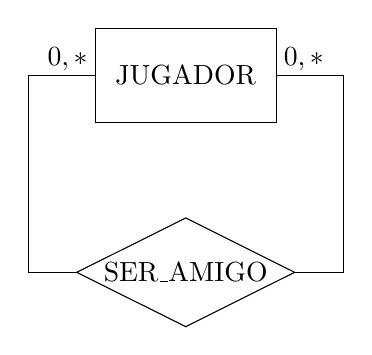
\begin{tikzpicture}
        \node[entity, minimum width=2.3cm, minimum height=1.2cm] (jugador) at (0,0) {JUGADOR};
        \node[relationship, aspect=2] (seramigo) at (0,-2.5) {SER\_AMIGO};
        \draw (seramigo.east) -- (2,-2.5) -- (2,0) -- (jugador.east);
        \draw (seramigo.west) -- (-2,-2.5) -- (-2,0) -- (jugador.west);
        \node at (-1.5,0.2) {$0 , \ast$};
        \node at (1.5,0.2) {$0,\ast$};

    \end{tikzpicture}
\end{frame}


\begin{frame}{Interrelaci\'on binaria}
    \begin{center}
        \Large{
            \textcolor{orange}{jugador} \hspace{10mm} \textcolor{blue}{coleccionar} \hspace{10mm} \textcolor{orange}{carta}
        }
    \end{center}
    \vspace{3mm}

    \centering
    
\begin{tikzpicture}
        \tikzstyle{every entity} = [minimum width=2.3cm, minimum height=1.2cm]
        \node[entity] (jugador) at (0,0) {JUGADOR};
        \node[entity] (carta) at (9,0) {CARTA};
        \node[relationship, aspect=2] (coleccionar) at (4.5,0) {COLECCIONAR} edge(jugador) edge(carta);
        \node at (7.5,0.2) {$1,\ast$};
        \node at (1.5,0.2) {$0,\ast$};
    \end{tikzpicture}
\end{frame}

\begin{frame}{Interrelaci\'on ternaria}
    \begin{overlayarea}{\linewidth}{\textheight}
        \vspace{5mm}
        \begin{center}
            \Large{
                \textcolor{orange}{jugador} \hspace{10mm} \textcolor{blue}{donar} \hspace{10mm} \textcolor{orange}{carta} \hspace{10mm} \textcolor{orange}{clan}
            }
        \end{center}
        \vspace{3mm}
    
        \centering
        \begin{tikzpicture}
            \tikzstyle{every entity} = [minimum width=2.3cm, minimum height=1.2cm]
            \node[entity] (jugador) at (0,0) {JUGADOR};
            \node[entity] (carta) at (9,0) {CARTA};
            \node[entity] (clan) at (4.5,-3) {CLAN};
            \node[relationship, aspect=2] (donar) at (4.5,0) {DONAR} edge(jugador) edge(carta) edge(clan);
            \onslide<3->{\node at (7.5,0.2) {$0,\ast$};}
            \onslide<5->{\node at (1.5,0.2) {$0,\ast$};}
            \onslide<7->{\node at (4.9,-2.2) {$0,1$};}
        \end{tikzpicture}
    
        \only<2>{
            \begin{block}{Cardinalidad en el extremo CARTA}
                ¿Un jugador puede donar a un clan cu\'antas cartas?
            \end{block}
        }
    
        \only<4>{
            \begin{block}{Cardinalidad en el extremo JUGADOR}
                ¿Una carta es donada a un clan por cu\'antos jugadores?
            \end{block}
        }
        \only<6>{
            \begin{block}{Cardinalidad en el extremo CLAN}
                ¿Un jugador puede donar una carta a cu\'antos clanes?
            \end{block}
        }
    \end{overlayarea}
\end{frame}

\begin{frame}{Interrelaci\'on unaria \only<2->{¿Seguros?}}
    \begin{overlayarea}{\linewidth}{\textheight}
        \vspace{6mm}
        \begin{center}
            \Large{
                \textcolor{orange}{jugador} \hspace{10mm} \textcolor{blue}{enfrentar} \hspace{10mm} \textcolor{orange}{jugador}
            }
        \end{center}
    
        \vspace{5mm}
    
        \centering
        \begin{tikzpicture}
            \node[entity, minimum width=2.3cm, minimum height=1.2cm] (jugador) at (0,0) {JUGADOR};
            \node[relationship, aspect=2] (enfrentar) at (0,-2.5) {ENFRENTAR};
            \draw (enfrentar.east) -- (2,-2.5) -- (2,0) -- (jugador.east);
            \draw (enfrentar.west) -- (-2,-2.5) -- (-2,0) -- (jugador.west);
            \node at (-1.5,0.2) {$0 , \ast$};
            \node at (1.5,0.2) {$0,\ast$};
    
            
            \only<3>{
                \node[align=left] at (6,-1) {
                    \{{\color<3>{red}(Pedro, Juan)}, {\color<3>{red}(Pedro, Juan)}, ... \}
                };
            }
        \end{tikzpicture}
    
    
        \vspace{3mm}
    
        \only<2>{¿Qu\'e ocurre si dos jugadores se enfrentan m\'as de una vez?}
        \only<3>{\textcolor{red}{Se crear\'ian instancias duplicadas en el conjunto de interrelaciones. Imposible}}
    \end{overlayarea}
\end{frame}

\begin{frame}{Interrelaciones en el tiempo}
    
    \centering
    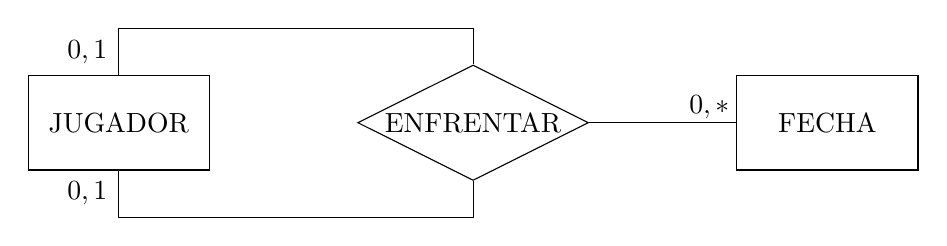
\begin{tikzpicture}
        \tikzstyle{every entity} = [minimum width=2.3cm, minimum height=1.2cm]
        \node[entity] (jugador) at (0,0) {JUGADOR};
        \node[entity] (fecha) at (9,0) {FECHA};
        \node[relationship, aspect=2] (enfrentar)at (4.5,0) {ENFRENTAR} edge(fecha);
        \draw (jugador.south) -- (0,-1.2) -- (4.5,-1.2) -- (enfrentar.south); 
        \draw (jugador.north) -- (0,1.2) -- (4.5,1.2) -- (enfrentar.north); 

        \node at (-0.4,0.9) {$0,1$};
        \node at (-0.4,-0.9) {$0,1$};
        \node at (7.5,0.2) {$0,\ast$};
    \end{tikzpicture}

    \vspace{5mm}

    \centering
        \{
            (Pedro, Juan, 24/02/23-14:55),
            (Pedro, Juan, 24/02/23-16:00),
            ...
        \}


\end{frame}


    
{
    \setbeamertemplate{background}{
        
\includegraphics[width=\paperwidth, height=\paperheight]{img/pls_stop.jpg}
    }
    \begin{frame}
    \end{frame}
}


{
    \setbeamertemplate{background}{
        
\includegraphics[width=\paperwidth, height=\paperheight]{img/nocatmeme.jpg}
    }
    \begin{frame}
    \end{frame}
}
    \begin{frame}{¿Hasta d\'onde hemos llegado?}
    \centering
    \resizebox{!}{7.5cm}{
    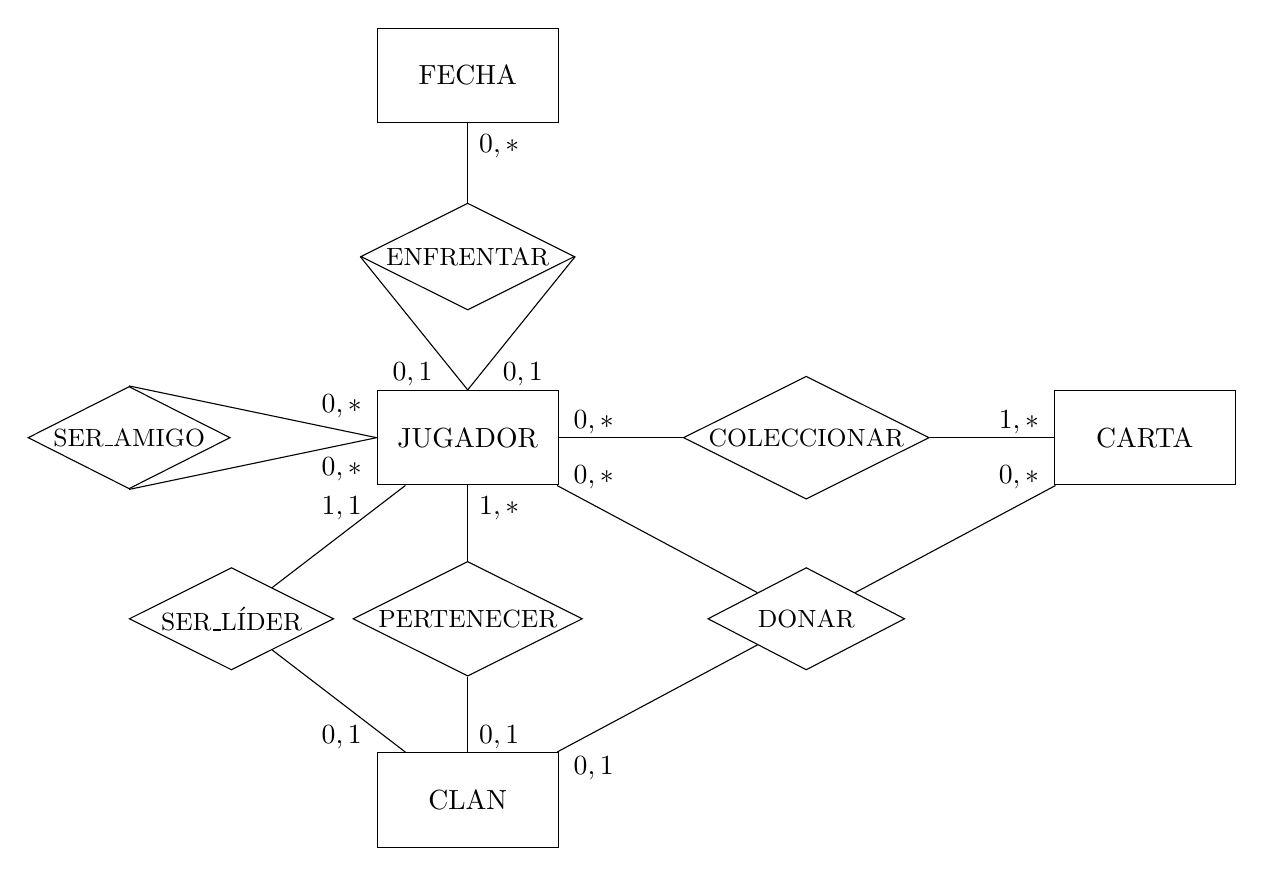
\begin{tikzpicture}
        \tikzstyle{every entity} = [minimum width=2.3cm, minimum height=1.2cm]
        \tikzstyle{every relationship} = [minimum width=2.5cm, minimum height=1.3cm]

        \node[entity] (jugador) at (0,0) {JUGADOR};
        \node[entity] (fecha) at (0,4.6) {FECHA};
        \node[entity] (clan) at (0,-4.6) {CLAN};
        \node[entity] (carta) at (8.6,0) {CARTA};

        \node[relationship,aspect=2] (pertenecer) at (0,-2.3) {\small PERTENECER}
            edge(jugador) edge(clan);
        \node at (0.4,-0.9) {$1,\ast$};
        \node at (0.4,-3.8) {$0,1$};


        \node[relationship,aspect=2] (coleccionar) at (4.3,0) {\small COLECCIONAR}
            edge(carta) edge(jugador);
        \node at (1.6,0.2) {$0,\ast$};
        \node at (7.0,0.2) {$1,\ast$};

        \node[relationship,aspect=2] (enfrentar) at (0,2.3) {\small ENFRENTAR}
            edge(fecha);
        \draw (enfrentar.west) -- (jugador.north);
        \draw (enfrentar.east) -- (jugador.north);
        \node at (0.7,0.8) {$0,1$};
        \node at (-0.7,0.8) {$0,1$};
        \node at (0.4,3.7) {$0,\ast$};

        \node[relationship,aspect=2] (seramigo) at (-4.3, 0) {\small SER\_AMIGO};
        \draw (seramigo.north) -- (jugador.west);
        \draw (seramigo.south) -- (jugador.west);
        \node at (-1.6,-0.4) {$0,\ast$};
        \node at (-1.6,0.4) {$0,\ast$};
      

        \node[relationship,aspect=2] (serlider) at (-3,-2.3) {\small SER\_L\'IDER}
            edge(jugador) edge(clan);
        \node at (-1.6,-3.8) {$0,1$};
        \node at (-1.6,-0.9) {$1,1$};
    

        \node[relationship,aspect=2] (donar) at (4.3,-2.3) {\small DONAR}
            edge(jugador) edge(clan) edge(carta);
        \node at (1.6,-4.2) {$0,1$};
        \node at (1.6,-0.5) {$0,\ast$};
        \node at (7,-0.5) {$0,\ast$};




        
    \end{tikzpicture}
    }
\end{frame}
    \begin{frame}{A\~nadiendo estructura}
    De cada {\color<2>{orange}jugador} se conoce su {\color<2>{attr}carnet de identidad}, 
    {\color<2>{attr}nombre}, 
    {\color<2>{attr}nivel}, la 
    {\color<2>{attr}cantidad de trofeos que tiene actualmente} y el 
    {\color<2>{attr}m\'aximo de trofeos que ha alcanzado}.
\end{frame}


% \begin{frame}{Atributo}

%     \begin{columns}[T]

%         \begin{column}{0.5\linewidth}
%             \begin{tikzpicture}
%                 \tikzstyle{every entity} = [minimum width=2cm, minimum height=0.8cm]
%                 \node[entity] (jugador) at (0,-4) {\small JUGADOR};
%                 \node[entity] (email) at (-2,2) {\small CI};
%                 \node[entity] (apodo)at (2,2) {\small NOMBRE};
        
%                 \node[relationship, aspect=2] (identificar) at (-2,-1) {\small IDENTIFICAR} edge(jugador) edge(email);
%                 \node[relationship] (tener) at (2,-1) {\small TENER} edge(jugador) edge(apodo);
        
%                 \node at (-2.4,1.3) {$1,{\color<2>{red}1}$};
%                 \onslide<2>{\draw[->,thick,color=red] (-2.6,0.6) -- (-2.3,1.1);}
%                 \node at (2.4,1.3) {${\color<5>{red}0},{\color<2>{red}1}$};
%                 \onslide<2>{\draw[->,thick,color=red] (3,0.6) -- (2.7,1.1);}
%                 \onslide<5>{\draw[->,thick,color=red] (2.6,0.5) -- (2.3,1.1);}

        
%                 \node at (-0.9,-3.4) {$1,{\color<3>{red}1}$};
%                 \onslide<3>{\draw[->,thick,color=red] (-1.5,-2.8) -- (-0.8,-3.2);}
%                 \node at (0.9,-3.4) {$1,{\color<4>{red}\ast}$};
%                 \onslide<4>{\draw[->,thick,color=red] (1.7,-2.6) -- (1.2,-3.2);}
        
        
%             \end{tikzpicture}
%         \end{column}

%         \begin{column}{0.48\linewidth}
%             \vspace{20mm}
%             \only<1>{
%                 \begin{block}{Definici\'on formal}
%                     Es una interrelaci\'on entre el conjunto
%                     de entidades de inter\'es y un conjunto de entidades que representa el atributo.
%                 \end{block}
%             }
%             \only<2-5>{
%                 \begin{alertblock}{Consideraciones importantes}
%                     \only<2> {Las cardinalidades m\'aximas en el extremo de los atributos siempre es 1}
%                     \only<3> {Existen atributos cuyo valor es \'unico para cada instancia del conjunto de entidades de inter\'es}
%                     \only<4> {Existen atributos que pueden tener el mismo valor para varias instancias del conjunto de entidades de inter\'es}
%                     \only<5> {Una instancia puede no tener valor asociado para un atributo, en cuyo caso el atributo es nulo}     
%                 \end{alertblock}

%             }
           
%         \end{column}
        
%     \end{columns}
    
% \end{frame}

\begin{frame}{Atributo}
    \begin{columns}[T]
        \begin{column}{0.5\linewidth}
            \centering
            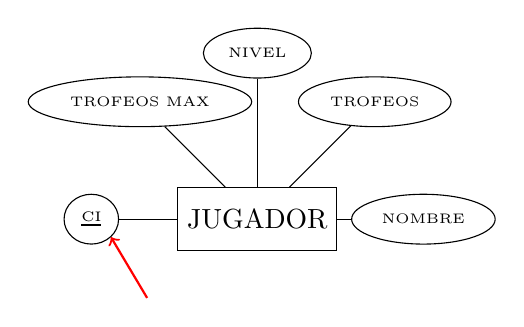
\begin{tikzpicture}[node distance=6em]
                \tikzstyle{every entity} = [minimum width=2cm, minimum height=0.8cm]

                \node[entity] (jugador) {JUGADOR}
                    [sibling distance=3cm]
                    child {node[attribute] [above left of=jugador] {\tiny TROFEOS MAX}}
                    child {node[attribute] [above right of=jugador]{\tiny TROFEOS}}
                    child {node[attribute] [above of=jugador] {\tiny NIVEL}}
                    child {node[attribute] [right of=jugador]{\tiny NOMBRE}}
                    child {node[attribute] (ci) [left of=jugador] {\tiny \underline{CI}}};

                \only<3>{

                    \draw[<-,thick,color=red] (ci.south east) -- (-1.4,-1);
                }
            \end{tikzpicture}

          
        \end{column}
        \begin{column}{0.48\linewidth}
            \vspace{10mm}
            \begin{block}{Definici\'on informal}
                Es una propiedad de un tipo de entidades.
            \end{block}
        \end{column}
    \end{columns}

    \only<2>{
        \vspace{5mm}
        \small {JUGADOR = \{
        (98012300205, Juan, 1, 1800, 2300), 
        (97041223987, Pedro, 3, 1600, 1800),
        (99072392022, Mar\'ia, 5, 1900, 2500),... 
        \}}
    }
   
    \only<3>{
    \vspace{5mm}

    \centering
    ¿Por qu\'e el carnet de identidad est\'a subrayado?
    }
\end{frame}


\begin{frame}{Atributo llave}
    \begin{block}{Problema}
        ¿C\'omo saber si en los conjuntos de entidades o conjuntos de interrelaciones existen
        instancias repetidas?
    \end{block}

    \begin{block}<2->{Soluci\'on}
        \begin{itemize}
            \item<2-> Una llave es un valor que siempre puede utilizarse de forma
            un\'ivoca para identificar una instancia dentro de un conjunto de instancias.
            \item<3-> La llave de un conjunto de entidades es una concatenaci\'on de una selecci\'on de sus atributos.
            \item<4-> La llave
            de un conjunto de interrelaciones es una concatenaci\'on de las llaves de
            los conjuntos entidades que intervienen en la relaci\'on.
        \end{itemize}
       
    \end{block}
\end{frame}

\begin{frame}{Estructurando los conjuntos de entidades}
    \begin{block}{}
        Las {\color<2->{orange}cartas} tienen un {\color<2->{attr}identificador}, un {\color<2->{attr}nombre}, una {\color<2->{attr}descripci\'on}, 
        un {\color<2->{attr}costo de elixir}  y una {\color<2->{attr}calidad} (común,
        especial, épica o legendaria).
    \end{block}
    \vspace{5mm}

    \onslide<3>{
    \centering
    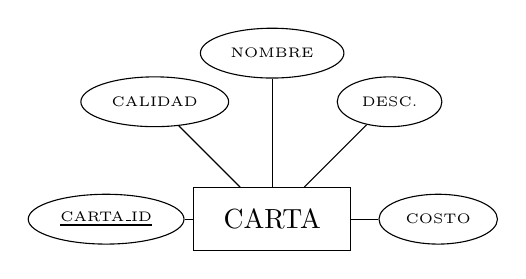
\begin{tikzpicture}[node distance=6em]
        \tikzstyle{every entity} = [minimum width=2cm, minimum height=0.8cm]

        \node[entity] (carta) {CARTA}
            [sibling distance=3cm]
            child {node[attribute] [above left of=carta] {\tiny CALIDAD}}
            child {node[attribute] [above right of=carta]{\tiny DESC.}}
            child {node[attribute] [above of=carta] {\tiny NOMBRE}}
            child {node[attribute] [right of=carta]{\tiny COSTO}}
            child {node[attribute] [left of=carta] {\tiny \underline{CARTA\_ID}}};
    \end{tikzpicture}
    }
\end{frame}

\begin{frame}{Estructurando los conjuntos de entidades}
    \begin{block}{}
        De los {\color<2->{orange}clanes} se conoce su {\color<2->{attr}identificador}, {\color<2->{attr}nombre}, una {\color<2->{attr}regi\'on}, 
        un {\color<2->{attr}tipo} (solo invitaci\'on o abierto)  y una {\color<2->{attr}cantidad m\'inima de trofeos} para entrar.
    \end{block}
    \vspace{5mm}

    \onslide<3>{
    \centering
    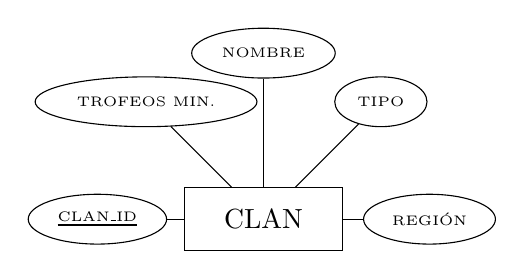
\begin{tikzpicture}[node distance=6em]
        \tikzstyle{every entity} = [minimum width=2cm, minimum height=0.8cm]

        \node[entity] (clan) {CLAN}
            [sibling distance=3cm]
            child {node[attribute] [above left of=clan] {\tiny TROFEOS MIN.}}
            child {node[attribute] [above right of=clan]{\tiny TIPO}}
            child {node[attribute] [above of=clan] {\tiny NOMBRE}}
            child {node[attribute] [right of=clan]{\tiny REGI\'ON}}
            child {node[attribute] [left of=clan] {\tiny \underline{CLAN\_ID}}};
    \end{tikzpicture}
    }

    \note<3>{@NOTE dudas?}
\end{frame}

% @TODO corta aki' la conf y ponle ejercicios. 


    \begin{frame}{¿Qu\'e otros escenarios ser\'ia interesante modelar?}
    \begin{block}{}
        Dentro de los {\color<2>{orange}jugadores} existen dos clases especiales de jugadores:
        \begin{itemize}
            \item   Los {\color<2>{orange}jugadores premium}
             son aquellos que se han gastado dinero en el juego, de estos se almacena
            la {\color<2>{attr}cantidad de dinero que han gastado} y su m\'etodo de pago preferido.

            \item  Los {\color<2>{orange}jugadores profesionales} son aquellos que {\color<2>{blue}son miembros} de un
            {\color<2>{orange}equipo profesional} y de ellos se almacena su {\color<2>{attr}ranking}.
        \end{itemize}
        De un equipo profesional se conoce su {\color<2>{attr}identificador}, 
        {\color<2>{attr}nombre} y {\color<2>{attr}pa\'is} de origen.
      
        
     
    \end{block}
\end{frame}


    % @NOTE for the next conf on thursday
    % {
    \setbeamertemplate{background}{
        
\includegraphics[width=\paperwidth, height=\paperheight]{img/mercy.jpg}
    }
    \begin{frame}
    \end{frame}
}


{
    \setbeamertemplate{background}{
        
\includegraphics[width=\paperwidth, height=\paperheight]{img/evil.jpg}
    }
    \begin{frame}
    \end{frame}
}

    % \begin{frame}{Por fin...}
    \begin{block}{Propuesta de E. F. Codd (1970)}
        \begin{itemize}
            \item Relacionar los datos mediante v\'inculos
            naturales, l\'ogicos, inherentes a los datos y al fen\'omeno y no
            a su representaci\'on computacional. 
            \item Lograr un modelo simple en el que tanto los datos
            como los v\'inculos que se establecen entre ellos se representen
            mediante tablas.
        \end{itemize}
        
    \end{block}
\end{frame}


\begin{frame}{¿Est\'an listos chicos?}
    
\includegraphics[width=\linewidth, height=0.85\textheight]{img/relational_model.jpg}
\end{frame}
    % \begin{frame}{¿Hasta d\'onde hemos llegado?}
    \centering
    \resizebox{14cm}{7.5cm}{
    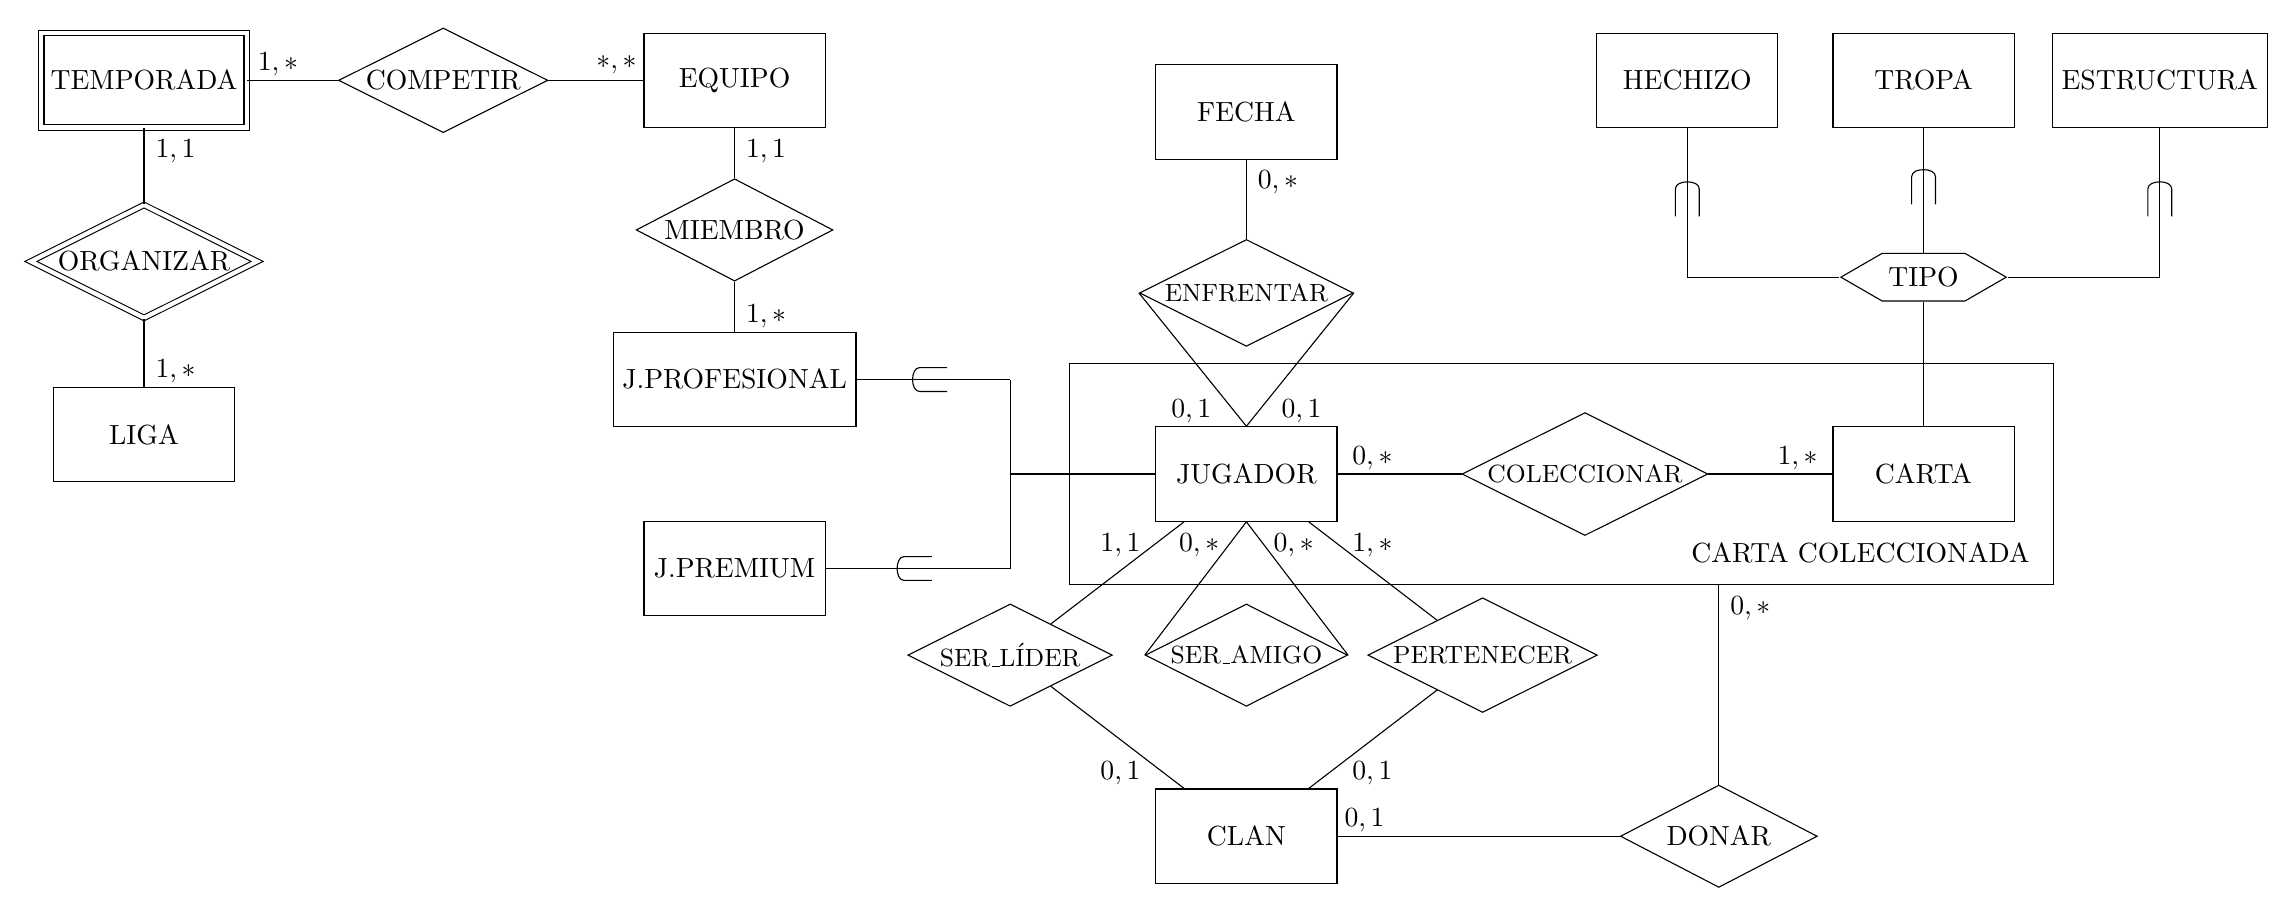
\begin{tikzpicture}
        \tikzstyle{every entity} = [minimum width=2.3cm, minimum height=1.2cm]
        \tikzstyle{every relationship} = [minimum width=2.5cm, minimum height=1.3cm]
        \tikzset{link/.append style={
            postaction={decorate},
            decoration={
                markings,
                mark= at position 0.5 with {
                    \draw (0.5em,1ex) -- (-0.5em,1ex) to[bend right=90] (-0.5em,-1ex) -- (0.5em,-1ex);
                }
            }
        }}
        \node[entity] (jugador) at (0,0) {JUGADOR};
        \node[entity] (fecha) at (0,4.6) {FECHA};
        \node[entity] (clan) at (0,-4.6) {CLAN};
        \node[entity] (carta) at (8.6,0) {CARTA};

        

        \node[entity] (tropa) at (8.6, 5) {TROPA};
        \node[entity] (estructura) at (11.6,5) {ESTRUCTURA};
        \node[entity] (hechizo) at (5.6,5) {HECHIZO};

        \node[regular polygon, draw, regular polygon sides=6, minimum width=7mm, xscale=3, label=center:TIPO] (tipo) at (8.6,2.5) {};
        \draw (carta.north) -- (tipo.south);
        \draw (tipo.west) -- (5.6,2.5);
        \draw (tipo.east) -- (11.6,2.5);
        \draw[link] (tropa.south) -- (tipo.north);
        \draw[link] (hechizo.south) -- (5.6,2.5);
        \draw[link] (estructura.south) -- (11.6,2.5);


        \node[relationship,aspect=2] (pertenecer) at (3,-2.3) {\small PERTENECER}
            edge(jugador) edge(clan);
        \node at (1.6,-0.9) {$1,\ast$};
        \node at (1.6,-3.8) {$0,1$};

        \node at (1.5,-4.4) {$0,1$};
        \node at (6.4,-1.7) {$0,\ast$};

        \node at (0.6,-0.9) {$0,\ast$};
        \node at (-0.6,-0.9) {$0,\ast$};

        \node[relationship,aspect=2] (coleccionar) at (4.3,0) {\small COLECCIONAR}
            edge(carta) edge(jugador);
        \node at (1.6,0.2) {$0,\ast$};
        \node at (7.0,0.2) {$1,\ast$};

        \node[relationship,aspect=2] (enfrentar) at (0,2.3) {\small ENFRENTAR}
            edge(fecha);
        \draw (enfrentar.west) -- (jugador.north);
        \draw (enfrentar.east) -- (jugador.north);
        \node at (0.7,0.8) {$0,1$};
        \node at (-0.7,0.8) {$0,1$};
        \node at (0.4,3.7) {$0,\ast$};

        \node[relationship,aspect=2] (seramigo) at (0, -2.3) {\small SER\_AMIGO};
        \draw (seramigo.east) -- (jugador.south);
        \draw (seramigo.west) -- (jugador.south);

        \node[relationship,aspect=2] (serlider) at (-3,-2.3) {\small SER\_L\'IDER}
            edge(jugador) edge(clan);
        \node at (-1.6,-3.8) {$0,1$};
        \node at (-1.6,-0.9) {$1,1$};

        \node[rectangle, draw, minimum width=12.5cm, minimum height=2.8cm] at (4,0) {};
        \node at (7.8,-1) {CARTA COLECCIONADA};

        \node[relationship, aspect=2] (donar) at (6,-4.6) {DONAR} edge(clan);
        \draw (6,-1.4) -- (donar.north);

        
        \draw (-3,0) -- (jugador.west);
        
        \node[entity] (premium) at (-6.5,-1.2) {J.PREMIUM};
        \node[entity] (profesional) at (-6.5,1.2) {J.PROFESIONAL};
        \draw (-3,0) -- (-3,-1.2);
        \draw (-3,0) -- (-3,1.2);
        \draw[link] (premium.east) -- (-3,-1.2);
        \draw[link] (profesional.east) -- (-3,1.2);


        \node[entity] (equipo) at (-6.5,5) {EQUIPO};
        \node at (-6.1,4.1) {$1,1$};
        \node at (-6.1,2) {$1,\ast$};

        \node[relationship,aspect=2] (miembro) at (-6.5,3.1) {MIEMBRO} edge(profesional) edge(equipo); 

        \node[entity,double distance=1.5pt] (temporada) at (-14, 5) {TEMPORADA};


        \node[entity] (liga) at (-14,0.5) {LIGA};
        \node[relationship,aspect=2,double distance=1.5pt] (organizar) at (-14,2.7) {ORGANIZAR} edge(temporada) edge(liga);

        \node[relationship,aspect=2] (compet) at (-10.2,5) {COMPETIR} edge(temporada) edge(equipo);
        
        \node at (-8,5.2) {$\ast,\ast$};
        \node at (-12.3,5.2) {$1,\ast$};

        \node at (-13.6,4.1) {$1,1$};
        \node at (-13.6,1.3) {$1,\ast$};
       
        



        
    \end{tikzpicture}
    }
\end{frame}

\begin{frame}{¿De d\'onde partimos?}
    \centering
    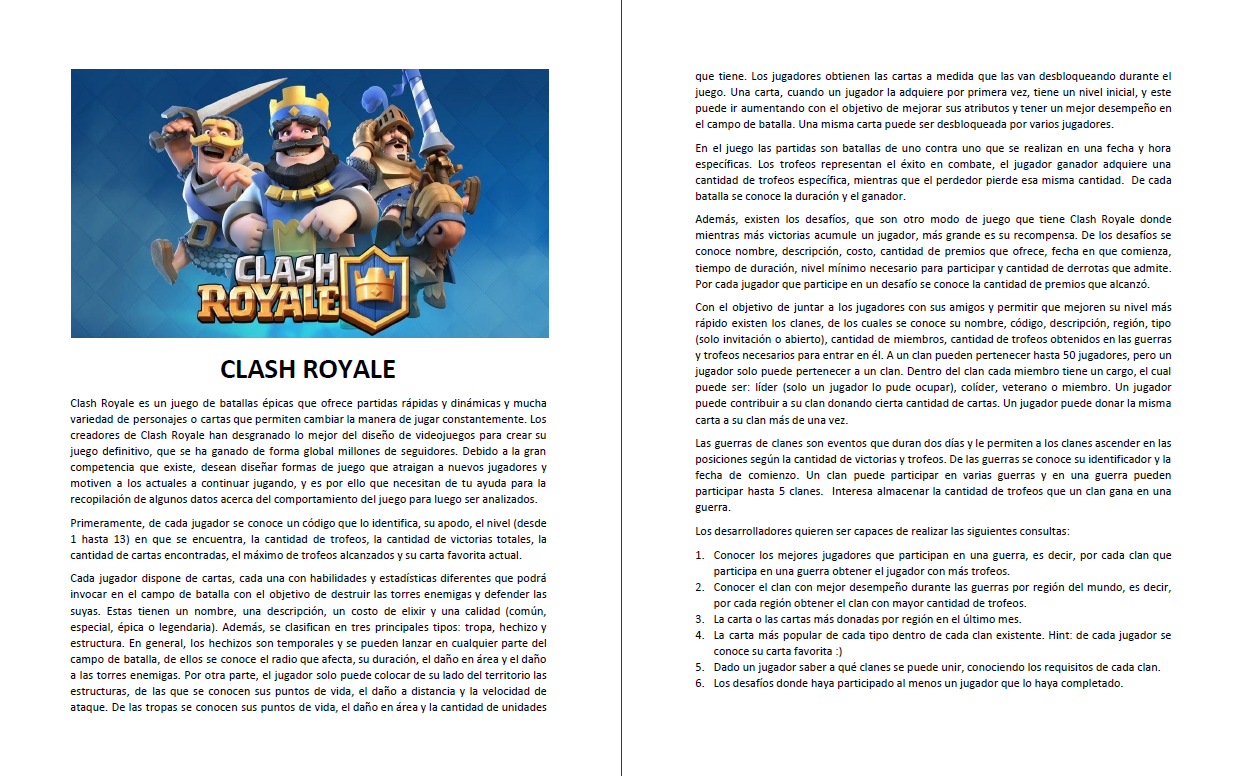
\includegraphics[width=0.8\linewidth, height=0.8\textheight]{img/specs.png}
\end{frame}

\begin{frame}{¿C\'omo obtener una especificaci\'on?}
    \begin{block}{An\'alisis de requerimientos}
        \begin{itemize}
            \item Descripciones en lenguaje natural
            \item Encuestas
            \item Observaci\'on directa 
            \item Formatos de registros
            \item Esquemas de datos
        \end{itemize}
    \end{block}
\end{frame}
    % \begin{frame}{¿Este MERX permite...}
    \begin{enumerate}
        \item ...conocer el resultado de un enfrentamiento?
        \item ...asegurar que los jugadores solo puedan donar cartas al clan que pertenecen?
        \item ...saber qué enfrentamientos ocurrieron en cada temporada de una liga profesional?
        \item ...asegurar que el líder de un clan deba pertenecer al clan que lidera?
        \item ...conocer las cartas más utilizadas en enfrentamientos?
    \end{enumerate}

\end{frame}
    % end of note scope

    

\begin{frame}{MERX como representaci\'on intermedia}
    \begin{columns}[T]
        \begin{column}{0.48\linewidth}
            \vspace{25mm}

            \resizebox{\linewidth}{!}{
            
\begin{tikzpicture}
                \tikzstyle{every entity} = [minimum width=2.3cm, minimum height=1.2cm]
                \node[entity] (jugador) at (0,0) {JUGADOR};
                \node[entity] (carta) at (9,0) {CARTA};
                \node[relationship, aspect=2] (coleccionar) at (4.5,0) {COLECCIONAR} edge(jugador) edge(carta);
                \node at (7.5,0.2) {$1,\ast$};
                \node at (1.5,0.2) {$0,\ast$};
            \end{tikzpicture}
            }
        \end{column}

        \begin{column}{0.48\linewidth}
            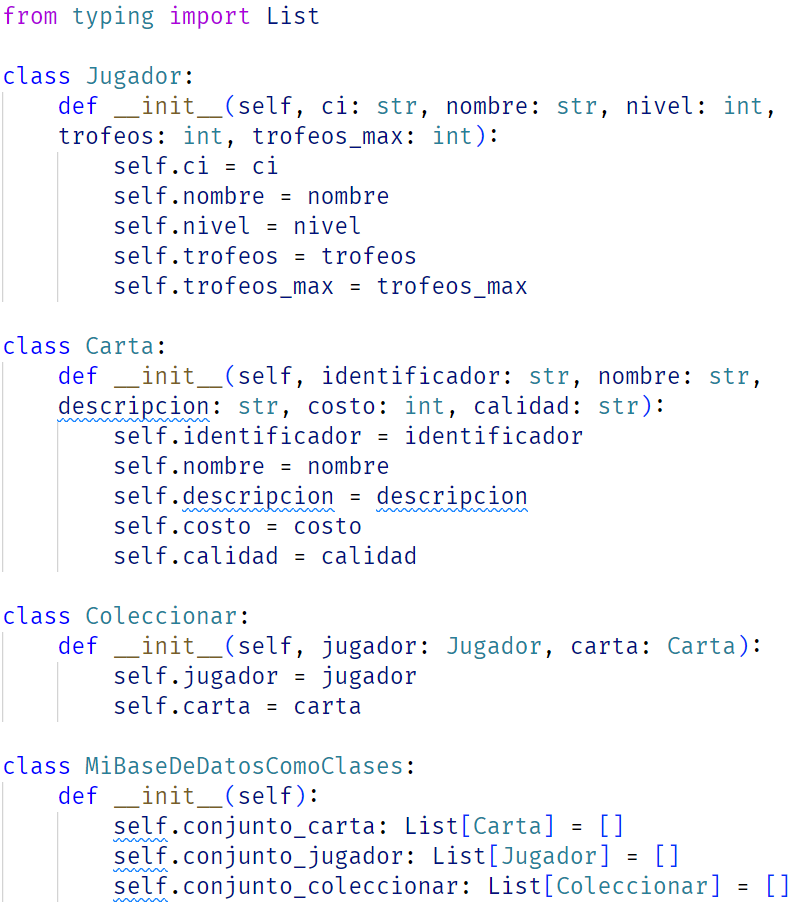
\includegraphics[width=0.9\linewidth, height=0.75\textheight]{img/classes.png}
        \end{column}
        
    \end{columns}
\end{frame}

\begin{frame}{MERX como representaci\'on intermedia}
    \begin{columns}[T]
        \begin{column}{0.48\linewidth}
            \vspace{25mm}

            \resizebox{\linewidth}{!}{
            
\begin{tikzpicture}
                \tikzstyle{every entity} = [minimum width=2.3cm, minimum height=1.2cm]
                \node[entity] (jugador) at (0,0) {JUGADOR};
                \node[entity] (carta) at (9,0) {CARTA};
                \node[relationship, aspect=2] (coleccionar) at (4.5,0) {COLECCIONAR} edge(jugador) edge(carta);
                \node at (7.5,0.2) {$1,\ast$};
                \node at (1.5,0.2) {$0,\ast$};
            \end{tikzpicture}
            }
        \end{column}


        \begin{column}{0.48\linewidth}
            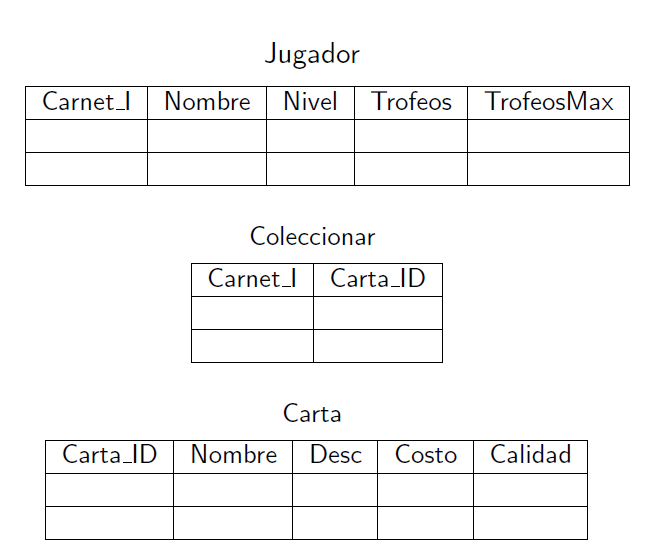
\includegraphics[width=\linewidth, height=0.75\textheight]{img/tables.png}
            % \centering
            % Jugador
            % \vspace{2mm}

            % \small
            % \begin{tabular}{|c|c|c|c|c|}
            %     \hline
            %     Carnet\_I & Nombre & Nivel & Trofeos & TrofeosMax\\
            %     \hline
            %     & & & &\\
            %     \hline
            %     & & & & \\
            %     \hline
            % \end{tabular}

            % \vspace{5mm}
            
            % \centering
            % Coleccionar
            % \vspace{2mm}
            
            % \begin{tabular}{|c|c|}
            %     \hline
            %     Carnet\_I & Carta\_ID \\
            %     \hline
            %     & \\
            %     \hline
            %     & \\
            %     \hline
            % \end{tabular}
            
            % \vspace{5mm}

            % \centering
            % Carta
            % \vspace{2mm}

            % \begin{tabular}{|c|c|c|c|c|}
            %     \hline
            %     Carta\_ID & Nombre & Desc & Costo & Calidad\\
            %     \hline
            %     & & & & \\
            %     \hline
            %     & & & & \\
            %     \hline
            % \end{tabular}
        \end{column}
        
    \end{columns}
\end{frame}
    
\begin{frame}{Entonces...}

    \begin{columns}[T]
        \begin{column}{0.4\linewidth}
            \vspace{3.3cm}

            \Huge ... alguna duda?
        \end{column}
        \begin{column}{0.58\linewidth}
            
            
\includegraphics[height=0.8\textheight, width=\linewidth]{img/eval.jpg}
        \end{column}
        
    \end{columns}
    
\end{frame}
    \begin{frame}
    \frametitle{Ejercicios}
    \framesubtitle<1>{1. Suministro de productos}
    \framesubtitle<2>{2. Pr\'estamo de libros}
    \framesubtitle<3>{3. Peque\~na cafetería}

    \only<1>{
        Se desea modelar el suministro de productos de una tienda. De cada suministrador se conoce su identificador, su nombre, su tipo y el municipio al que pertenece. De cada producto se conoce su c\'odigo, su nombre, su precio y la unidad de medida que le corresponde. Un suministrador suministra un producto en una cierta cantidad. Cada suministrador puede suministrar varios productos. Cada producto puede ser suministrado por varios suministradores.
    }
    \only<2>{
        En una librer\'ia se prestan libros a sus miembros. De cada libro se tiene registrado su t\'itulo, autor, ISBN, a\~no de publicaci\'on y g\'enero. Los miembros son usuarios de la librer\'ia y de ellos se conoce un identificador \'unico, el nombre, direcci\'on, tel\'efono y correo. Cuando un libro es prestado a un miembro se registra la fecha en la que fue emitido el pr\'estamo, la fecha en la que debe ser devuelto el libro y la fecha en la que realmente este se devolvi\'o. Cada pr\'estamo est\'a constituido por un solo libro y es emitido a nombre de un solo miembro.
    }
    \only<3>{
        En una pequeña cafetería de barrio los clientes visitan para comprar café y pasteles. Cada cliente posee una identificación única y puede acumular puntos de fidelidad. Se realizan pedidos, cada uno con un ID de pedido único, que comprende varios productos como café y pasteles. Los productos tienen sus propios ID, nombres, tipos y precios. Los empleados, incluidos barman y gerentes, son responsables de procesar los pedidos. Cada empleado tiene un ID, nombre, rol y turnos asignados. Los pedidos se rastrean por su estado, monto total y método de pago. 
    }

    \note<2>{@NOTE el ISBN es un c\'odigo \'unico para identificar un libro}
\end{frame}
    \maketitle
\end{document}
